
\subsubsection{Cellular and Wireless Communications}
\label{Haas1} \index{Haas, Harald}

\paragraph{Research Team}
Harald Haas (Professor), Rami Abu-Alhiga (PhD Student), Zubin Bharucha
(PhD Student), Hany Elgala (PhD Student), Ellina Foutekova (PhD
Student), Birendra Ghimire (PhD Student), Dennis Kolyuzhnov (PhD
Student),  Raed Youself Mesleh (PhD Student), Abdurazak Mudesir (PhD
Student), Hrishikesh Venkataraman (PhD Student), Sinan Sinanovic
(Research Associate), Peter Omiyi (Postdoctoral Fellow), Mostafa
Afgani (Research Engineer), Sudharasan Ganesan (MSc student)\\

Research in Cellular and Wireless Communications is geared towards new
technologies for wireless systems. Particular focus is placed on the
development and the interaction of key air-interface building blocks:
\begin{myitemize}
\item multicarrier transmission (in particular OFDM (Orthogonal Frequency Division Multiplexing),
\item duplexing techniques (in particular time division duplexing (TDD)),
\item multiple-input multiple-output (MIMO) techniques,
\item wireless ad hoc systems,
\item medium access control (MAC) algorithms,
\item multiple access and scheduling techniques,
\item dynamic channel assignment (DCA) algorithms,
\item mobile positioning
\item visible light communication
\end{myitemize}

\myparagraph{Highlights}
\emph{1. Spatial Modulation:}
Spatial modulation (SM) is a new and patented multiple antenna
transmission approach for wireless systems that increases the spectral
efficiency (number of bits transmitted per Hz bandwidth) by utilizing
the transmit antenna number as an implicit source of information. A
block of information bits is mapped to an information symbol and a
transmit antenna number. As a consequence, at any given time instant
only a single antenna of the antenna array is transmitting signal
power. The actual block of information bits determines which antenna
is active at a particular time instant. As a result, inter-channel
interference (ICI) at the receiver input and the need to synchronize
the transmit antennas are completely avoided. Simple receiver
algorithms such as maximum receive ratio combining (MRRC) can be used
to retrieve the information bits. The performance and the receiver
complexity of SM and V-BLAST (Vertical-Bell Labs Layered Space-Time)
algorithm in flat fading channels are compared. V-BLAST applies zero
forcing detection based optimum ordering, nulling and successive
interference cancellation. The basic principle of SM is depicted in Fig.~\ref{smexmpl}, and results of the comparison with state-of-the-art V-BLAST are shown in Fig.~\ref{fig55}.
\begin{figure}[!htb]\centering
  \centerline{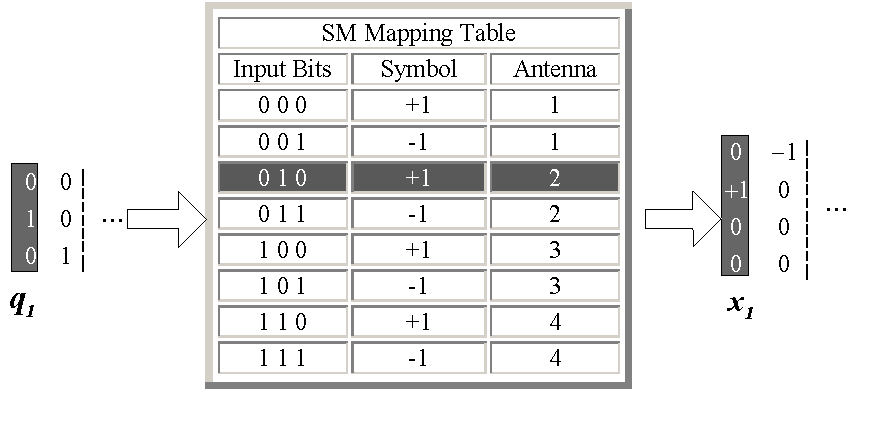
\includegraphics[width=8cm]{haas_1.pdf}}
  \caption{3bits/symbol spatial modulation mapping table using binary phase shift keying (BPSK)
    and four transmit antennas} \label{smexmpl}
\end{figure}
\begin{figure}[!!htp]\centering
  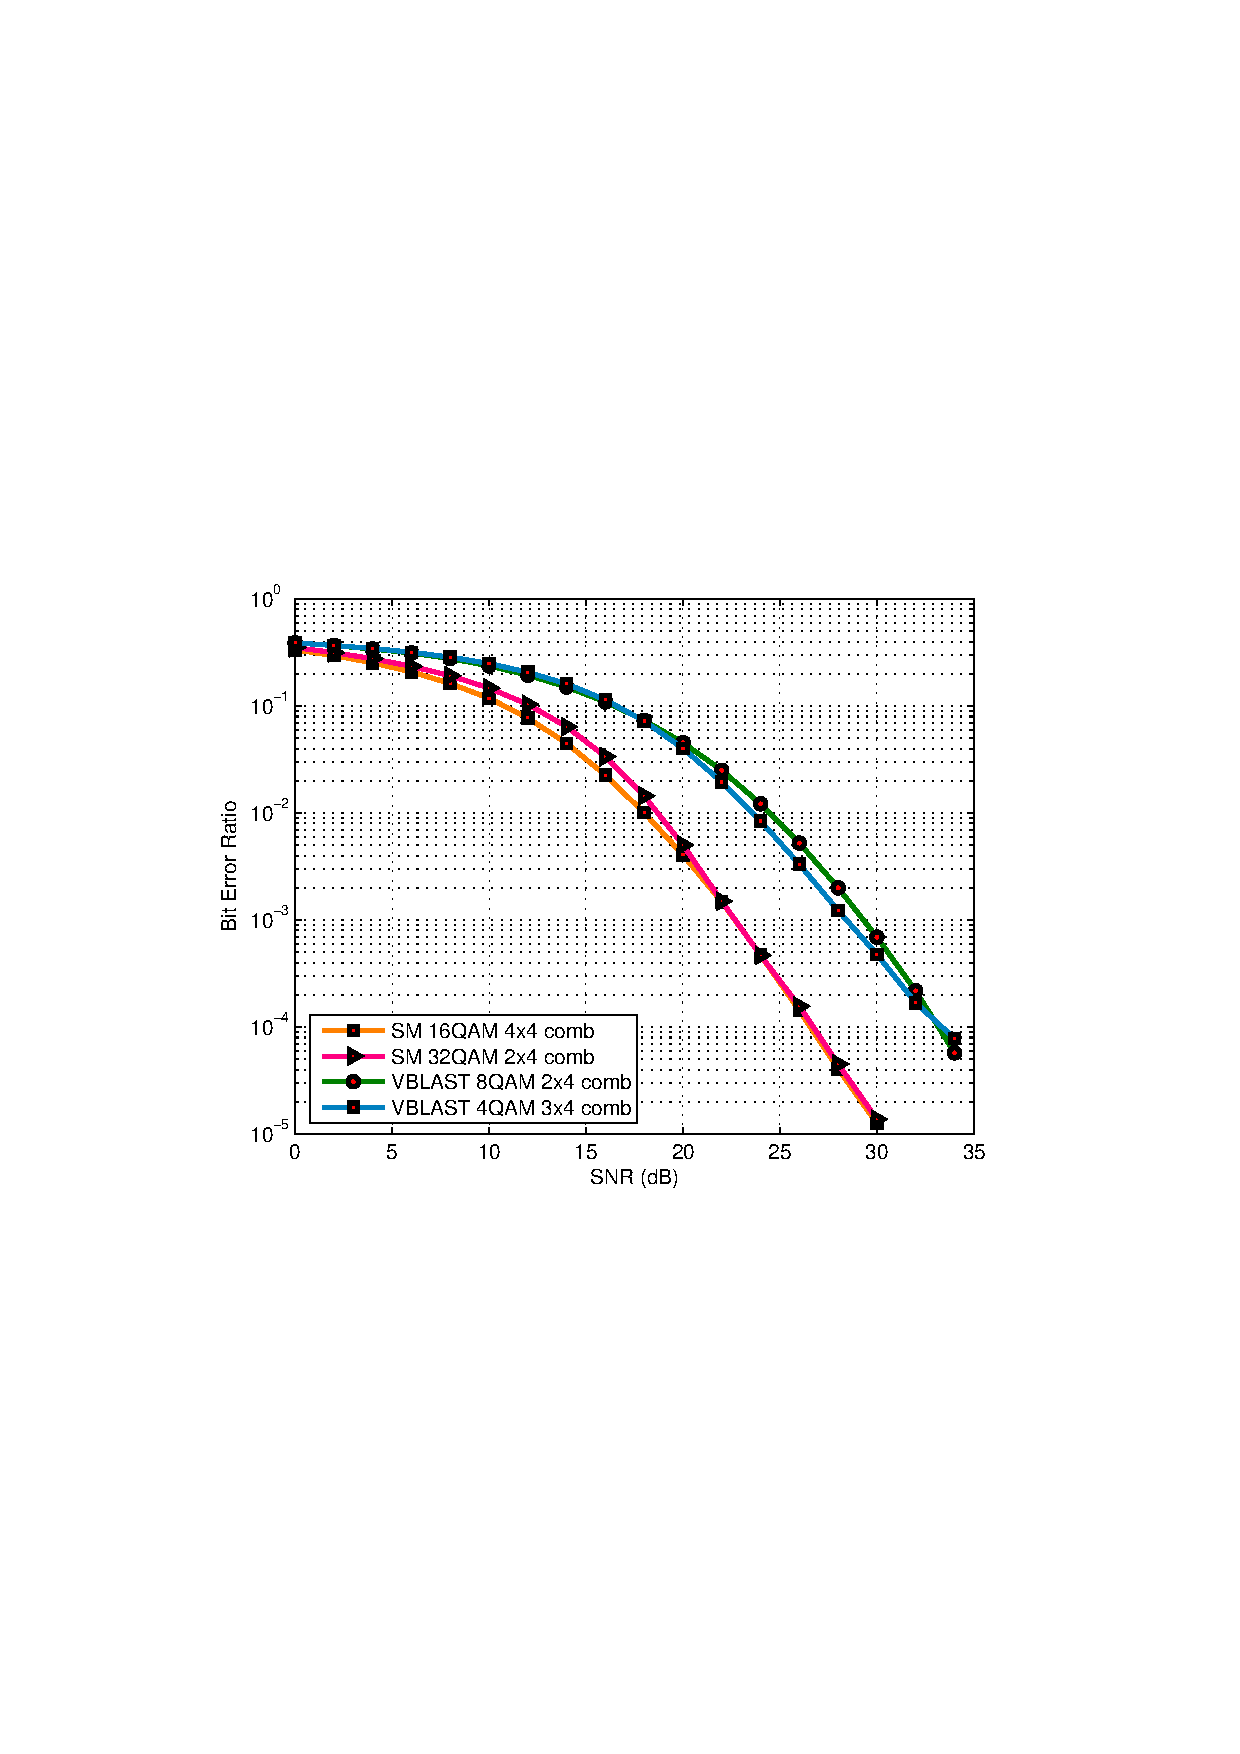
\includegraphics[width=8cm]{haas_2.pdf}\\
  \caption{Bit error performance as a function of signal-to-noise ratio (SNR) for state-of-the-art V-BLAST and novel SM.}
  \label{fig55}
\end{figure}
From the results it can be found that the performance gains are
significant. In both schemes the same number of bit per unit bandwidth
are transmitted (for fair comparison), but with SM the bit error performance is reduced
considerably. For example, at an SNR of 20dB a 10-fold reduction in
the BER is observed.\\

\emph{2. Dynamic Resource Allocation:}
In this work a fully decentralized interference avoidance algorithm to
manage interference in an \emph{ad hoc} wireless network, applicable
to wireless sensor networks, is developed and analyzed. Fig.~\ref{dca}
depicts a randomly chosen distribution of transmitting (Tx) and
receiving (Rx) nodes. The new algorithm, called \emph{busy tone
interference tolerance signaling}, is of low complexity and is very
easy to implement. It is based on different functions to set the busy tone
signal power dependent on the level of tolerable interference, and
their performance is compared with a special case of a fixed power
system which provides maximum capacity assuming equal transmit
powers. Results show that an appropriately chosen function for setting
the busy-tone can lead to gains in capacity using very little
power. This power efficiency advantage is quite significant, implying
that battery life of units can be extended while providing a similar
capacity than a fixed power system.
\begin{figure}[!!htp]
 \centering
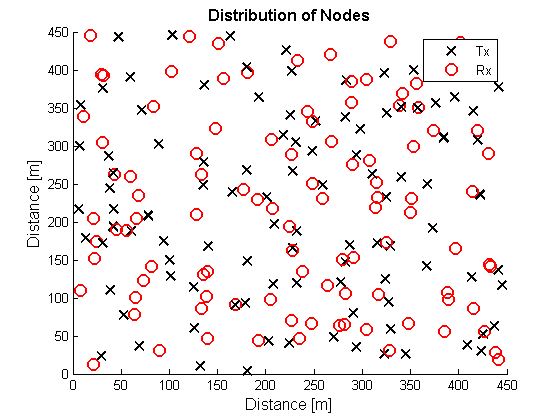
\includegraphics[width=8cm]{haas_3.png}\\
\caption{Random distribution of nodes in an \emph{ad hoc} wireless network}
\label{dca}
\end{figure}

%\null Harald Haas is also involved in ``Signal Processing''
%(Section~\ref{Haas1}).

%\newpage
\paragraph{Organization}
% list the (research) events you have organized, if any,
\begin{enumerate}
    \item Member of Technical Program Committee of and session chair
          at \emph{IEEE International Conference on Personal, Indoor \& Mobile Radio Communications} -- PIMRC 2006
    \item Member of Technical Program Committee of \emph{International IEEE Conference on Vehicular Technology} -- VTC 2006
\end{enumerate}

\paragraph{Collaborations}
\begin{enumerate}
\item {\sl The University of Edinburgh, UK}\\
  Prof. Stephen McLaughlin\\
  Joint project with industrial partner on \emph{Hybrid Cellular and Multihop Wireless
    Networks}
\end{enumerate}


\paragraph{Grants}
% list the running grants in 2005, if none have been received, please delete this
% subsection.
\begin{enumerate}
    \item Funded by industry partner,
      \emph{Cellular TDD-OFDM (Time division duplex - orthogonal frequency
          division multiplexing)}, (June 2004 - July 2005)\\


    \item Funding by industry partner and University of Edinburgh, \emph{Hybrid Cellular and Multihop Wireless
    Networks}, (July 2005 - July 2006)

    \item Funded by industry partner, \emph{Link Adaptation and Scheduling in Cellular
    Systems}, (March 2005 - February 2008)\\

    \item Funded by Bremen T.I.M.E program funded by BIS
    Bremerhaven, \emph{Mobile Positioning (MPos)} in collaboration with MobilTec GmbH and supported by
     T-Mobile, (June 2006 - September 2009)

    \item Funded by DFG Schwerpunktprogram TakeOFDM (322-1163) \emph{DCA Algorithms and MAC Protocols for COFDM Based Cellular and
     Ad hoc Systems Using Carrier Sensing Time Division Multiple Access
     (CSTDMA)}, (October 2004 - September 2006)
     
\end{enumerate}

\paragraph{Patents}
% list the grants you have received in 2005, if none have been received, please delete this
% subsection.
\begin{enumerate}
\item Four new patent applications submitted
\item Three previously submitted patents got granted in 2006
\end{enumerate}

\paragraph{Awards, Prizes}
\begin{enumerate}
\item Nominated for the Chinese 111 Program -- Guest Academic Talents Programme for the Development of University Disciplines in China
\item Invited Talk at the University of Mondragon (Spain)
%    \item Honorary Fellowship of Edinburgh University
%    \item Invited to Institute for Digital Communications (IDCOM) at the University of
%          Edinburgh on \emph{Vodafone Fellowship on Communications}
    %\item Invited speaker at \emph{International Next Generation Wireless Network Workshop},
     %     Edinburgh/Scotland
\end{enumerate}

\newpage
%\paragraph{Publications}
% list the publications of 2005 (also accepted and in press), if none have been received, please delete this
% subsection. Enter the publications into the SES publications database at
% http://kwarc.eecs.iu-bremen.de/ses-pubs/index.php and only reference them here.

%\begin{description}
%  \item[Conference Proceedings]
\nocite{ah06_vis_light}
\nocite{bh06_ped_dead_reck}
\nocite{hnona06_iamac}
\nocite{vh06_thru_cap}
\nocite{cvh06_freq_syn}
\nocite{feh06_semi_analytic}
\nocite{fagvh06_sch_CDMA}
\nocite{jhm06_adhoc_tdd_underlay}
\nocite{oha06_tsalloc_insotdd}
\nocite{mhay06_spatialmod}
\nocite{asilomar06}
\nocite{chinacom06}
%\item[Books/Collections]
\nocite{tdd_book}
\nocite{oha07}
%\end{description}

%\bibliographystyle{IEEEtran}
%\bibliography{macros,report}
%\end{document}
%%% Local Variables:
%%% mode: latex
%%% TeX-master: "report"
%%% End:

% LocalWords:  Harald optimisation Multicarrier OFDM Duplexing duplexing TDD SM
% LocalWords:  MIMO DCA intercellular timeslot TDMA minislot neighbouring haas
% LocalWords:  pdf pathloss timeslots Pollaczek Khinchin TPC PIMRC Keio Masao
% LocalWords:  Nakagawa Riaz Esmailzadeh IUB otz Pfander kEURO IDCOM Vodafone
% LocalWords:  organiser Rami Abu Alhiga Zubin Bharucha Hany Elgala Ellina Raed
% LocalWords:  Foutekova Birendra Ghimire Kolyuzhnov Youself Mesleh Abdurazak
% LocalWords:  Mudesir Hrishikesh Venkataraman Sinan Sinanovic Omiyi Mostafa dB
% LocalWords:  Afgani multicarrier utilizing ICI synchronize MRRC nulling BPSK
% LocalWords:  SNR BER decentralized analyzed Tx Rx signaling Organization VTC
% LocalWords:  organized Multihop BIS Bremerhaven MPos MobilTec GmbH DFG COFDM
% LocalWords:  Schwerpunktprogram TakeOFDM CSTDMA
